\documentclass[journal]{IEEEtran}

\usepackage{cite}
\usepackage{float}
\usepackage{graphicx}
\usepackage[caption=false]{subfig}
  \DeclareGraphicsExtensions{.png}
\usepackage{amsmath}
\usepackage{amsfonts}
\usepackage{url}

\hyphenation{photo-graphed diff-erence}

\begin{document}

\title{%
  High-radix On-line Arithmetic Verification System\\
  \large Final Year Project 1800478: Interim Report}
\author{Zifan Wang, 01077639\\Imperial College London}

% \markboth{2018-2019}{?}

\maketitle

% \begin{abstract}
% \end{abstract}

% --------------------------------------------------------------------------------
% --------------------------------------------------------------------------------
\section{Introduction}
% The Interim report should normally be between 10 and 30 pages long. Remember
% that it must be a project planning document for the remainder of your project
% work, as well as being an early write-up of your background material. Using
% Interim Report material, without explicit reference, in your Final Report is
% allowed, and even encouraged. The Interim Report is often a first draft of the
% background section of the Final Report. Self-plagiarism, in this case, is not an
% issue. It is expected that you will reuse Interim Report material without
% explicit reference.

This project is a part of a larger project investigating the effect of using
high-radix number systems with on-line arithmetic operators.
The overarching aim would involve implementing such a system on FPGA and
quantifying its performance improvements.
This aim would be achieved through two vertically split individual projects.
One would design and verify the arithmetic operator modules,
while the other would design a system from the top-level to test and
evaluate these operators.
This project deals with the system-level issues.

% --------------------------------------------------------------------------------
% --------------------------------------------------------------------------------
\section{Project Specification}
% The project specification should state clearly what the project is intended to
% deliver, including all hardware, software, simulation, and analytical work, and
% provide some motivation.

As this project progresses in parallel with the designing of the operator
modules, it is necessary to decouple the two project so that as individual
projects, they are individually evaluated.
The success of one project should not be restricted by the status of the other.
To this end, the goal of the system-level design is more focussed on its
functionalities and robustness.
This relationship and its effect on the evaluation will be examined further in
the evaluation chapter of this report.

\subsection{Project Interfacing}
% REVISIT: necessary? if already decided, what is it?
A number representation system should be decided before detailed design starts.

The modules would be compiled hardware in 

\subsection{Deliverables}
At the end of the project, the system should be able to perform the following:
\begin{enumerate}
  \item Takes in the arithmetic modules designed by the sister project as its
        input;
  \item Generate and run tests on these modules;
  \item Vary the frequency and voltage of the FPGA;
  \item Evaluate its performance.
\end{enumerate}

\subsection{Hardware Choice}
The system itself will be built on a Cyclone V SX SoC Development Board from
Intel~\cite{Cy5DBWeb}.

\begin{figure}[H]
  \centering
  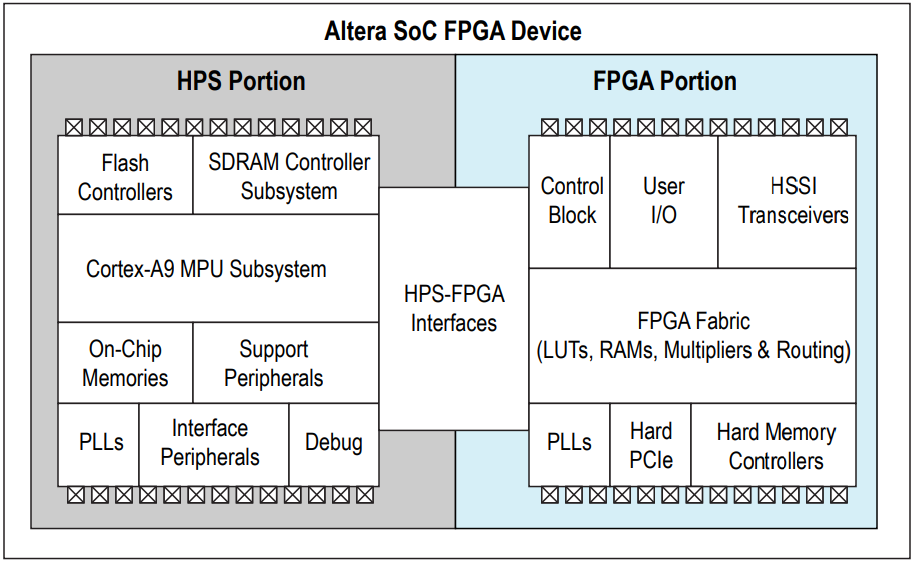
\includegraphics[width=8cm]{img/SoCStructure}
  \caption{Structure of the System-on-Chip}
  \label{SoCStructure}
\end{figure}

The 5CSXFC6D6F31C6N SoC has a Am Cortex-A9 MPCore accompanied by Intel's 28nm
FPGA fabric~\cite{Cy5DBRM}.
The FPGA is necessary for implementing the hardware design and obtaining
empirical results for the project.
% REVISIT: is this true? why do we need an HPS?
Having an HPS on the same chip is useful as the test software can run on it,
allowing a better user interface to be constructed with more detailed,
on-the-fly control to the FPGA.

It should be noted that Xilinx offers similar boards as well. Its Zynq SoC
family has a very comparable structure as they too integrate the software
programmability of an Arm processor with the hardware possibility of an FPGA.
For example, like the Cyclone V SX, Zynq-7000S also features a Arm Cortex-A9
coupled with a Xilinx 28nm FPGA~\cite{ZynqBrief}.

% REVISIT: need to show evidence for their similarity?
As there are very few significant functional differences between the two brands,
this project will initially explore with the Intel board, simply for its
availability and the personal familiarity with their development tools.

Once the project has progressed to a point where the system design is mature and
tested, the Xilinx alternative could be explored as an extension.

\subsection{Software Choice}
The software choice follows closely with the hardware choice in this project.
To develop for Intel FPGA, Quartus needs to be used.
% REVISIT: are you sure about this one?
The version picked is arbitrary as there is not much functional difference
between the versions that would be critical to the project.
As Quartus Prime 16.0 is the version installed in the computers in the
department.
The project will be using the same version for the convenience.
This naturally means the hardware system will be build with the system
integration tool that comes with Quartus -- Qsys.

Other than the hardware design tools, there are some freedom of choice in the
HPS side of the project.
The test will be build with Python, which will be running on an Ubuntu system
that is installed in the HPS.
This choice is made for there are previous unrelated projects on the same
develop board that uses the same configuration, which means a lot of time
could be saved on getting an operating system booting.

\subsection{Deliverables}
The initial deliverable for the engineering side involves running a simple
program on the FPGA through the HPS with the FPGA frequency being controllable.
After this, the next critical step would be making sure the modules under test
will be the point of failure and not the testbench.
This would include some research on ways in improving the speed of feeding
inputs to the arithmetic units, and checking its outputs.
Once this could be confirmed, we can start adding a selection of different functionalities.

\begin{enumerate}
  \item Running standard benchmarks;
  \item Running key algorithms or their components;
  \item Experiment with other power efficiency improving techniques,
        such as undervolting;
  \item Add support for different radix arithmetic;
  \item Allow graceful failures for the testbench in case of unintended
        behaviour for the arithmetic modules;
  \item Add an interactive UI to control the voltage and frequency at run time
        and examine the DUT’s behaviour;
\end{enumerate}

Depending on the time situation, more or less items on this list may be fulfilled.

\subsection{Evaluation Metric}

% --------------------------------------------------------------------------------
% --------------------------------------------------------------------------------
\section{Background}
% The background section must outline the necessary background to the project,
% stating how it is important for the project work. For example: survey of related
% literature, analysis of competing products, technical specifications of hardware
% or software standards, electronic components, necessary software tools,
% background theory. The contents of this section will vary for different
% projects, and in many cases the background reading will have been completed –
% but if not you should be in a position to list what remains to be done (e.g. a
% set of research papers to read and understand). A good benchmark of progress
% here is that you have accumulated (though may not yet have read) at least 20
% references to background material. In projects which have substantial background
% writing up your literature survey in the Interim Report will save time at the
% end of the project and allow this element of your final report to receive timely
% feedback from your supervisor so the final write-up can be improved.

% explain online
% explain high-radix

% --------------------------------------------------------------------------------
% --------------------------------------------------------------------------------
\section{Implementation Plan}
% The implementation plan is a preliminary breakdown of the work that is to be
% done in the remainder of the project. You should identify a set of milestones
% and provide a realistic estimate of when each of these should be completed if
% all goes well. It should also detail fallback positions in case any stage of the
% development goes wrong. You may feel, in the early stages of your project work,
% that the times in this plan are guesses. However you will find as the project
% progresses that keeping track of and revising your initial estimates, and if
% necessary altering the proposed work, is a vital way to ensure that the project
% is finished in time. In projects with heavy implementation content you should
% document what you have already completed.

Compared to existing research, the combination of high-radix and online is
relatively novel, and to optimising it on a system level for popular FPGA
accelerations such as neural networks would be innovative as well.
With respect to the testbench, figuring out a system to obtain the optimal point
of operation of the FPGA, in terms of its voltage and frequency, would also
require some advanced research.

\subsection{Risks}
A major risk of this project is related to its schedule and the existence of an
initial blocking task.
While most of the later sections of the project can be selectively added or
removed from the scope relatively easily, the initial setup of the testbench
will always remain critical to any further improvements.
It is thus vital that the bare minimum system gets done early.
To ensure this happens, it will be placed in the highest priority before its
completion, and any blocking issue should be discussed with the supervisor if it
could not be resolved after significant effort.

The other major risk has to do with the progress of the sister project.
The purpose of the testbench is to verify and stress the arithmetic designs.
If these designs would not be available near the end of this project,
it would be difficult to empirically prove the capabilities of the testbench
and its surrounding system.
It is not impossible, as there are still substitutions for them.
For functional purposes, standard off-the-shelf adders and multipliers could be
used in-lieu.
For other purposes, it is possible to have a model done before the actual design
starts in the paired project.
While this would allow this project to progress easier, it would be extra work
for the other project, which is ultimately up to the decision of the other
student.
In all, it would be nice to have a solid arithmetic module completely to run
in this testbench, but without one, the system can still be built and completed,
albeit generating less useful data towards the overall aim of the project.

% --------------------------------------------------------------------------------
% --------------------------------------------------------------------------------
\section{Evaluation Plan}
% The evaluation plan should detail how you expect to measure the success of the
% project. In particular it should document any tests that are required to ensure
% that the project deliverable(s) function correctly, together with (where
% appropriate) details of experiments required to evaluate the work with respect
% to other products or research results.

% --------------------------------------------------------------------------------
% --------------------------------------------------------------------------------
\section{Ethical, Legal, and Safety Plan}
% The Ethical, Legal and Safety Plan must detail what are the issues in this are
% relevant to your project, showing how you will comply with best practice. If
% there are no such issues (the case for 80\% of all projects) you must
% nevertheless show here that you have considered these issues and detail why they
% will not apply to your project. Information will be provided on the project web
% pages about Ethical, Legal and Safety matters.

% --------------------------------------------------------------------------------
% --------------------------------------------------------------------------------
\section{Conclusion}

\newpage
\appendices

\section{Formulae}
$$1 + 1 = 2$$

\section{Data}

\begin{table}[H]
  \centering
  \begin{tabular}{c|cccc}
    Sum             & $1$ & $2$ & $3$ & $4$ \\
    \hline
    $1$             & $2$ & $3$ & $4$ & $5$ \\
    $2$             & $3$ & $4$ & $5$ & $6$ \\
  \end{tabular}
\end{table}

\section{Illustrations}

\begin{figure}[H]
  \centering
  
\includegraphics[width=8cm]{img/placeholder}
  \caption{Placeholder}
  \label{ph}
\end{figure}

\begin{thebibliography}{1}

\bibitem{Cy5DBWeb}
    Intel Corporation,
    ``\textit{Cyclone V SoC Development Kit and Intel SoC FPGA Embedded
    Development Suite}''.
    Available at: \url{intel.com/content/www/us/en/programmable/products/
    boards_and_kits/dev-kits/altera/kit-cyclone-v-soc.html}.

\bibitem{Cy5DBRM}
    Altera Corporation,
    ``\textit{Cyclone V SoC Development Board Reference Manual}'',
    2015.
    Available at: \url{intel.com/content/dam/www/programmable/us/en/pdfs/
    literature/manual/rm_cv_soc_dev_board.pdf}.

\bibitem{ZynqBrief}
    Xilinx, Inc,
    ``\textit{Zynq-7000 All Programmable SoC}'',
    2018.
    Available at: \url{https://www.xilinx.com/support/documentation/
    product-briefs/zynq-7000-product-brief.pdf}.

\end{thebibliography}

\end{document}